\documentclass[10pt]{article}
\usepackage{tikz}
\usetikzlibrary{arrows,shapes,plotmarks,backgrounds,trees,snakes,decorations.markings, calc}

\newcommand\TBox[3][]{%
\tikz\node[thick, rounded corners,  align=left,#1] at #3 {#2};\hskip2pt}

\begin{document}

\begin{center}
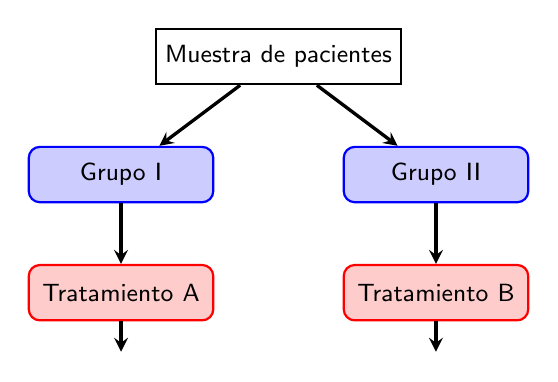
\begin{tikzpicture}[very thick,>=stealth,
grup/.style ={rectangle, draw=blue, thick, fill=blue!20, text width=6em,align=center, rounded corners, minimum height=2em},
tract/.style ={rectangle, draw=red, thick, fill=red!20, text width=6em,align=center, rounded corners, minimum height=2em},
origen/.style ={rectangle, draw=black, thick, align=center,minimum height=2em}
]
\draw (0,0) node[origen] (O) {\small \sf Muestra de pacientes};  
\draw (-2,-1.5) node[grup] (I) {\small \sf Grupo I};  
\draw (2,-1.5) node[grup] (II) {\small \sf Grupo II};  
\draw (-2,-3) node[tract] (A) {\small \sf Tratamiento A};  
\draw (2,-3) node[tract] (B) {\small \sf Tratamiento B};  
\draw[->] (O)--(I);
\draw[->] (O)--(II);
\draw[->] (I)--(A);
\draw[->] (II)--(B);
\draw[->] (A)--(-2,-3.75);
\draw[->] (B)--(2,-3.75);

\end{tikzpicture}
\end{center}
\vspace*{2cm}

\begin{center}
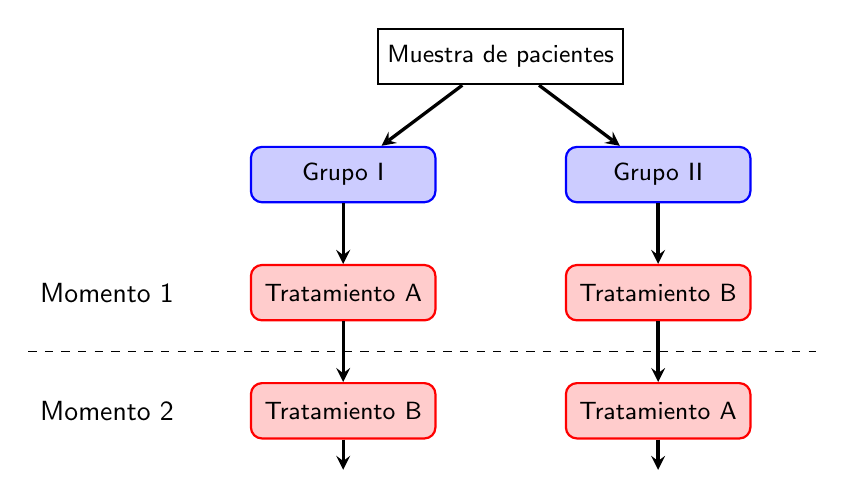
\begin{tikzpicture}[very thick,>=stealth,
grup/.style ={rectangle, draw=blue, thick, fill=blue!20, text width=6em,align=center, rounded corners, minimum height=2em},
tract/.style ={rectangle, draw=red, thick, fill=red!20, text width=6em,align=center, rounded corners, minimum height=2em},
origen/.style ={rectangle, draw=black, thick, align=center,minimum height=2em}
]
\draw (0,0) node[origen] (O) {\small \sf Muestra de pacientes};  
\draw (-2,-1.5) node[grup] (I) {\small \sf Grupo I};  
\draw (2,-1.5) node[grup] (II) {\small \sf Grupo II};  
\draw (-2,-3) node[tract] (A1) {\small \sf Tratamiento A};  
\draw (2,-3) node[tract] (B1) {\small \sf Tratamiento B};  
\draw (-2,-4.5) node[tract] (B2) {\small \sf Tratamiento B};  
\draw (2,-4.5) node[tract] (A2) {\small \sf Tratamiento A};  
\draw[->] (O)--(I);
\draw[->] (O)--(II);
\draw[->] (I)--(A1);
\draw[->] (II)--(B1);
\draw[->] (A1)--(B2);
\draw[->] (B1)--(A2);
\draw[->] (A2)--(2,-5.25);
\draw[->] (B2)--(-2,-5.25);
\draw[thin,dashed] (-6,-3.75)--(4,-3.75);
\draw (-5,-3) node {\sf Momento 1};  
\draw (-5,-4.5) node {\sf Momento 2};  
\end{tikzpicture}
\end{center}


\end{document}

\tikzstyle{vecArrow} = [thick, decoration={markings,mark=at position
   1 with {\arrow[semithick]{open triangle 60}}},
   double distance=1.4pt, shorten >= 5.5pt,
   preaction = {decorate},
   postaction = {draw,line width=1.4pt, white,shorten >= 4.5pt}]

\begin{center}
\begin{tikzpicture}[very thick,>=stealth,scale=0.5,block/.style ={rectangle, draw=blue, thick, fill=blue!20, text width=6em,align=center, rounded corners, minimum height=2em}]%,xscale=0.75]
\draw (10,0) node[block] (A) {\small \sf Enfermedad};  
\draw (0,1) node[block]   {\small\sf Expuestos\\[-0.5ex] \small\sf sanos}; 
\draw (0,-1) node[block]   {\small \sf No expuestos\\[-0.5ex] \small\sf sanos}; 
\draw[vecArrow] (2.3,0)--(A);
\end{tikzpicture}
\end{center}
\vspace*{2cm}

\begin{center}
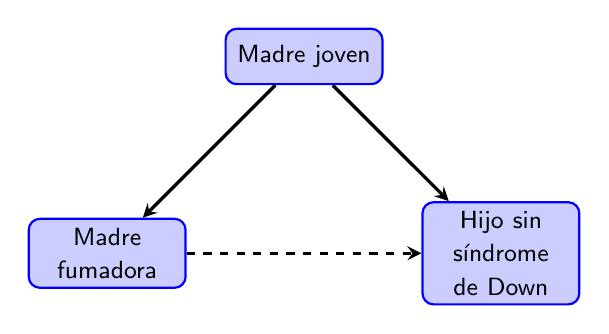
\begin{tikzpicture}[very thick,>=stealth,scale=0.5,block/.style ={rectangle, draw=blue, thick, fill=blue!20, text width=5em,align=center, rounded corners, minimum height=2em}]%,xscale=0.75]
\draw (0,0) node[block] (A) {\small\sf Madre fumadora};  
\draw (10,0) node[block] (B) {\small\sf Hijo sin síndrome de Down}; 
\draw (5,5) node {};
\draw[dashed,->] (A)--(B);
\draw(5,5) node[block] (C) {\small\sf Madre joven};
\draw[->] (C)--(A);
\draw[->] (C)--(B);
\end{tikzpicture}
\end{center}
\vspace*{2cm}


\begin{center}
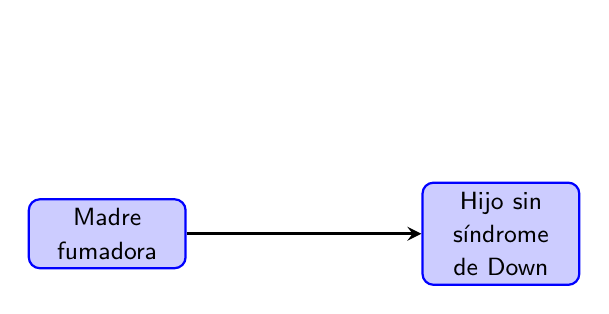
\begin{tikzpicture}[very thick,>=stealth,scale=0.5,block/.style ={rectangle, draw=blue, thick, fill=blue!20, text width=5em,align=center, rounded corners, minimum height=2em}]%,xscale=0.75]
\draw (0,0) node[block] (A) {\small\sf Madre fumadora};  
\draw (10,0) node[block] (B) {\small\sf Hijo sin síndrome de Down}; 
\draw (5,5) node {};
\draw[->] (A)--(B);
\end{tikzpicture}
\end{center}



\end{document}
\begin{center}
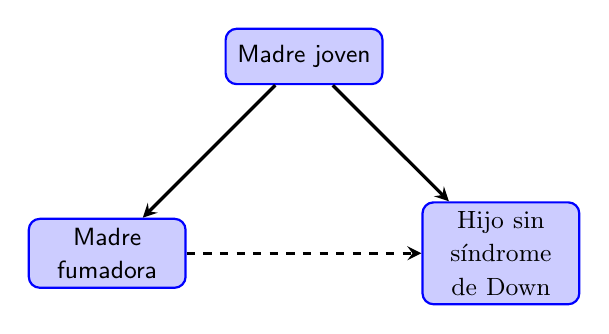
\begin{tikzpicture}[very thick,>=stealth,scale=0.5,block/.style ={rectangle, draw=blue, thick, fill=blue!20, text width=5em,align=center, rounded corners, minimum height=2em}]%,xscale=0.75]
\draw (0,0) node[block] (A) {\small\sf Madre fumadora};  
\draw (10,0) node[block] (B) {\small Hijo sin síndrome de Down}; 
\draw (5,5) node {};
\draw[dashed,->] (A)--(B);
\draw(5,5) node[block] (C) {\small\sf Madre joven};
\draw[->] (C)--(A);
\draw[->] (C)--(B);
\end{tikzpicture}
\end{center}


\end{document}

\begin{center}

\tikz\node[thick, rounded corners,  align=left,draw=green, fill=green!20] at (0,1){\textsf{\textbf{Descriptivos}}\\[2ex]
\tikz\node[thick, rounded corners,  align=left,draw= blue,fill=blue!20] at (0,1){\small\sf Informe de caso};
\\[1ex]
\tikz\node[thick, rounded corners,  align=left,draw= blue,fill=blue!20] at (0,0) {\small\sf Serie de casos};\\[1ex]
\tikz\node[thick, rounded corners,  align=left,draw= blue,fill=blue!20] at (0,-1) {\small \textsf{\textsl{Survey}}};};
\hspace*{0.5cm}
\tikz\node[thick, rounded corners,  align=left,draw=green, fill=green!20] at (3,0){\textsf{\textbf{Analíticos}}\\[2ex]
\tikz\node[thick, rounded corners,  align=left,draw=red, fill=red!20] at (3,0){\textsf{\textbf{Observacionales}}\\[2ex]
\tikz\node[thick, rounded corners,  align=left,draw= blue,fill=blue!20] at (3,0){\small\sf Casos y controles};
\\[1ex]
\tikz\node[thick, rounded corners,  align=left,draw= blue,fill=blue!20] at (3,-1) {\small\sf Cohorte};\\[1ex]
\tikz\node[thick, rounded corners,  align=left,draw= blue,fill=blue!20] at (3,-2) {\small\sf Transversal};\\[1ex]
\tikz\node[thick, rounded corners,  align=left,draw= blue,fill=blue!20] at (3,-3) {\small\sf Ecológico};};
\\[1ex]
\tikz\node[thick, rounded corners,  align=left,draw=red, fill=red!20] at (3,-4){\textsf{\textbf{Intervencionistas}}\\[2ex]
\tikz\node[thick, rounded corners,  align=left,draw= blue,fill=blue!20] at (3,-5) {\small\sf Experimental};\\[1ex]
\tikz\node[thick, rounded corners,  align=left,draw= blue,fill=blue!20] at (3,-5) {\small\sf Casi-experimental};};\\[1ex]
\tikz\node[thick, rounded corners,  align=left,draw=yellow, fill= yellow!20] at (3,-6){\textsf{\textbf{Metaanálisis \hphantom{xxxi}}}};};


\end{center}

\end{document}

\begin{center}
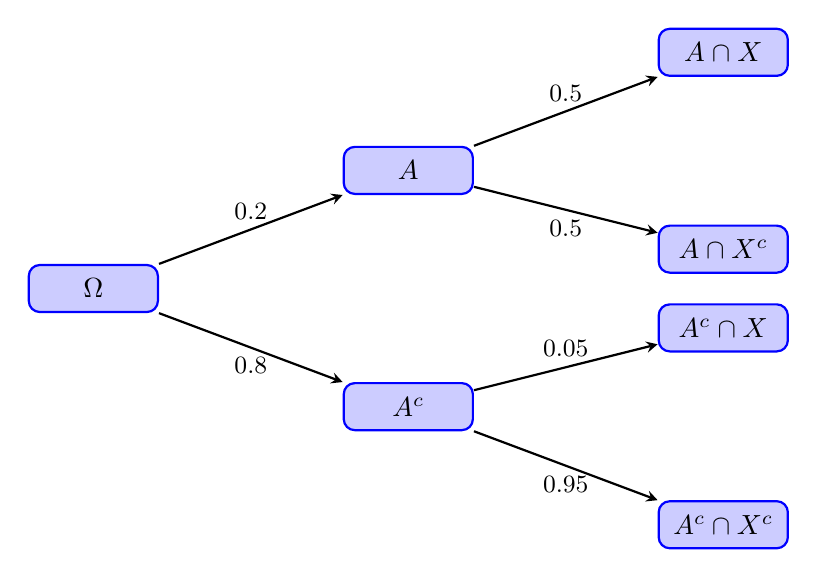
\begin{tikzpicture}[very thick,>=stealth,scale=0.5,block/.style ={rectangle, draw=blue, thick, fill=blue!20, text width=4em,align=center, rounded corners, minimum height=1.7em}]%,xscale=0.75]
\draw (0,0) node[block] (Omega) {$\Omega$};  
\draw (8,3) node[block] (A)   {$A$}; 
\draw (8,-3) node[block]  (Ac)  {$A^c$}; 
\draw (16,6) node[block] (AX)   {$A\cap X$}; 
\draw (16,1) node[block] (AXc)   {$A\cap X^c$}; 
\draw (16,-1) node[block] (AcX)   {$A^c\cap X$}; 
\draw (16,-6) node[block] (AcXc)   {$A^c\cap X^c$}; 
\draw [thick, ->] (Omega) -- (A) node[midway,above] {\small 0.2};
\draw [thick, ->] (Omega) -- (Ac) node[midway,below] {\small 0.8};
\draw [thick, ->] (A) -- (AX) node[midway,above] {\small 0.5};
\draw [thick, ->] (A) -- (AXc) node[midway,below] {\small 0.5};
\draw [thick, ->] (Ac) -- (AcX) node[midway,above] {\small 0.05};
\draw [thick, ->] (Ac) -- (AcXc) node[midway,below] {\small 0.95};

\end{tikzpicture}
\end{center}

\end{document}
\tikzstyle{vecArrow} = [thick, decoration={markings,mark=at position
   1 with {\arrow[semithick]{open triangle 60}}},
   double distance=1.4pt, shorten >= 5.5pt,
   preaction = {decorate},
   postaction = {draw,line width=1.4pt, white,shorten >= 4.5pt}]

\begin{center}
\begin{tikzpicture}[very thick,>=stealth,scale=0.5,block/.style ={rectangle, draw=blue, thick, fill=blue!20, text width=5em,align=center, rounded corners, minimum height=2em}]%,xscale=0.75]
\draw (0,0) node[block] (A) {\small\sf Exposición};  
\draw (10,1) node[block]   {\small \sf Enfermos}; 
\draw (10,-1) node[block]   {\small \sf Sanos}; 
\draw[vecArrow] (8,0)--(A);
\end{tikzpicture}
\end{center}
\vspace*{3cm}

\begin{center}
\begin{tikzpicture}[very thick,>=stealth,scale=0.5,block/.style ={rectangle, draw=blue, thick, fill=blue!20, text width=6em,align=center, rounded corners, minimum height=2em}]%,xscale=0.75]
\draw (10,0) node[block] (A) {\small \sf Enfermedad};  
\draw (0,1) node[block]   {\small\sf Expuestos}; 
\draw (0,-1) node[block]   {\small \sf No expuestos}; 
\draw[vecArrow] (2.3,0)--(A);
\end{tikzpicture}
\end{center}
\end{document}


\end{document}
%\TBox[draw= blue,fill=blue!20]{\small \textsf{\textsl{Survey}}}{(0,3)}\\[2.5ex]}{(0,0)}
%\hspace*{0.5cm}%
%\TBox[draw=red, fill=red!20]{\textsf{\textbf{Analíticos}}\\[2ex]
%\TBox[draw= blue,fill=blue!20]{\small\sf Casos y controles}\\[1ex]
%\TBox[draw= blue,fill=blue!20]{\small\sf Cohorte}\\[1ex]
%\TBox[draw= blue,fill=blue!20]{\small\sf Transversal}\\[1ex]
%\TBox[draw= blue,fill=blue!20]{\small\sf Ecológico}\\[-2ex]}
%\hspace*{0.5cm}%
%\TBox[draw=yellow, fill=yellow!20]{\textsf{\textbf{Metaanálisis}}}




\begin{center}
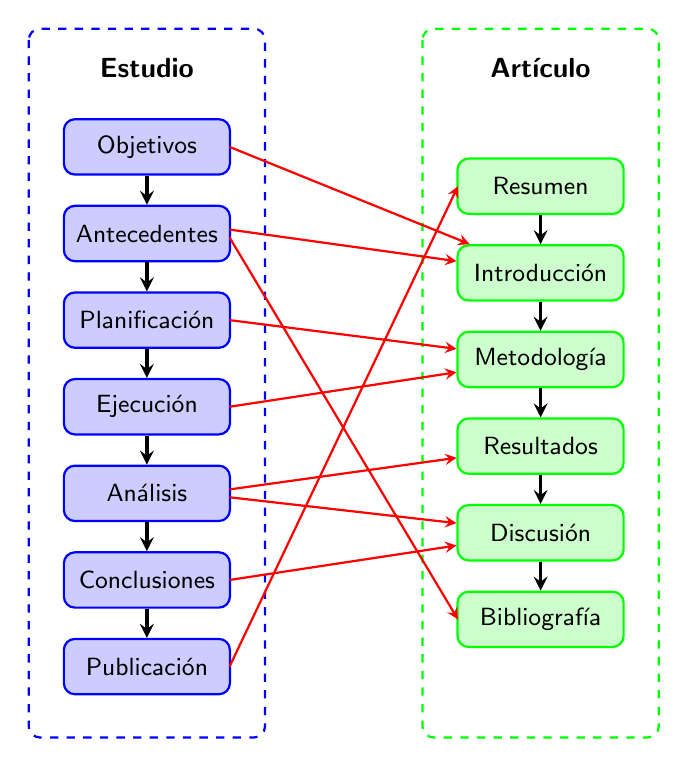
\begin{tikzpicture}[>=stealth,scale=1, very thick,
pas/.style ={rectangle, draw=blue, thick, fill=blue!20, align=center, rounded corners, minimum height=2em,minimum width=6em},
part/.style ={rectangle, draw=green, thick, fill=green!20, align=center, rounded corners, minimum height=2em,minimum width=6em}]

\draw (0,0) node[pas] (Ob) {\small\sf Objetivos};  
\draw (0,-1.1) node[pas] (Ant) {\small\sf Antecedentes};  
\draw (0,-2.2) node[pas] (Plan) {\small\sf Planificación};  
\draw (0,-3.3) node[pas] (Ej) {\small\sf Ejecución};  
\draw (0,-4.4) node[pas] (Anal) {\small\sf Análisis};  
\draw (0,-5.5) node[pas] (Conc) {\small\sf Conclusiones};  
\draw (0,-6.6) node[pas] (Pub) {\small\sf Publicación};  
\draw[->] (Ob)--(Ant);
\draw[->] (Ant)--(Plan);
\draw[->] (Plan)--(Ej);
\draw[->] (Ej)--(Anal);
\draw[->] (Anal)--(Conc);
\draw[->] (Conc)--(Pub);
\draw (0,1) node  {\textsf{\textbf{Estudio}}};  
\draw (5,1) node  {\textsf{\textbf{Artículo}}}; 
\draw[blue, thick,dashed, rounded corners] (-1.5,1.5)  rectangle (1.5,-7.5);
\draw[green, thick,dashed, rounded corners] (3.5,1.5)  rectangle (6.5,-7.5);




\draw (5,0-0.5) node[part] (Abs) {\small\sf Resumen};  
\draw (5,-1.1-0.5) node[part] (Intro) {\small\sf Introducción};  
\draw (5,-2.2-0.5) node[part] (Met) {\small\sf Metodología};  
\draw (5,-3.3-0.5) node[part] (Res) {\small\sf Resultados};  
\draw (5,-4.4-0.5) node[part] (Dis) {\small\sf Discusión};  
\draw (5,-5.5-0.5) node[part] (Bib) {\small\sf Bibliografía};  
\draw[->] (Abs)--(Intro);
\draw[->] (Intro)--(Met);
\draw[->] (Met)--(Res);
\draw[->] (Res)--(Dis);
\draw[->] (Dis)--(Bib);

\draw[thick,red,->] (1.05,0)--(Intro);
\draw[thick,red,->] (1.05,-1.05)--(Intro);
\draw[thick,red,->] (1.05,-1.15)--(3.95,-6);
\draw[thick,red,->] (1.05,-2.2)--(Met);
\draw[thick,red,->] (1.05,-3.3)--(Met);
\draw[thick,red,->] (1.05,-4.35)--(Res);
\draw[thick,red,->] (1.05,-4.45)--(Dis);
\draw[thick,red,->] (1.05,-5.5)--(Dis);
\draw[thick,red,->] (1.05,-6.6)--(3.95,-0.5);


\end{tikzpicture}



\end{center}


\end{document}

\begin{center}
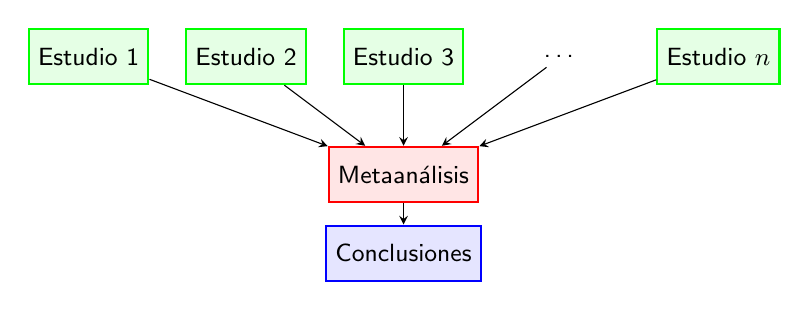
\begin{tikzpicture}[>=stealth,scale=1,
resp/.style={rectangle, draw=green, thick, fill=green!10, align=center,  minimum height=2em},
prestudy/.style={rectangle, draw=blue, thick, fill=blue!10, align=center,  minimum height=2em}]

\draw (-4,0) node[resp] (E1) {\small\sf Estudio 1};  
\draw (-2,0) node[resp] (E2) {\small\sf Estudio 2};  
\draw (0,0) node[resp] (E3) {\small\sf Estudio 3};  
\draw (2,0) node  (E4) {\small\sf \ldots};  
\draw (4,0) node[resp] (E5) {\small\sf Estudio $n$};  
\draw (0,-1.5) node[rectangle, draw=red, thick, fill=red!10, align=center,  minimum height=2em] (MA) {\small\sf Metaanálisis};  
\draw (0,-2.5) node[prestudy] (CC) {\small\sf Conclusiones};  


\draw[->] (E1)--(MA);
\draw[->] (E2)--(MA);
\draw[->] (E3)--(MA);
\draw[->] (E4)--(MA);
\draw[->] (E5)--(MA);
\draw[->] (MA)--(CC);
\end{tikzpicture}
\end{center}


\begin{center}
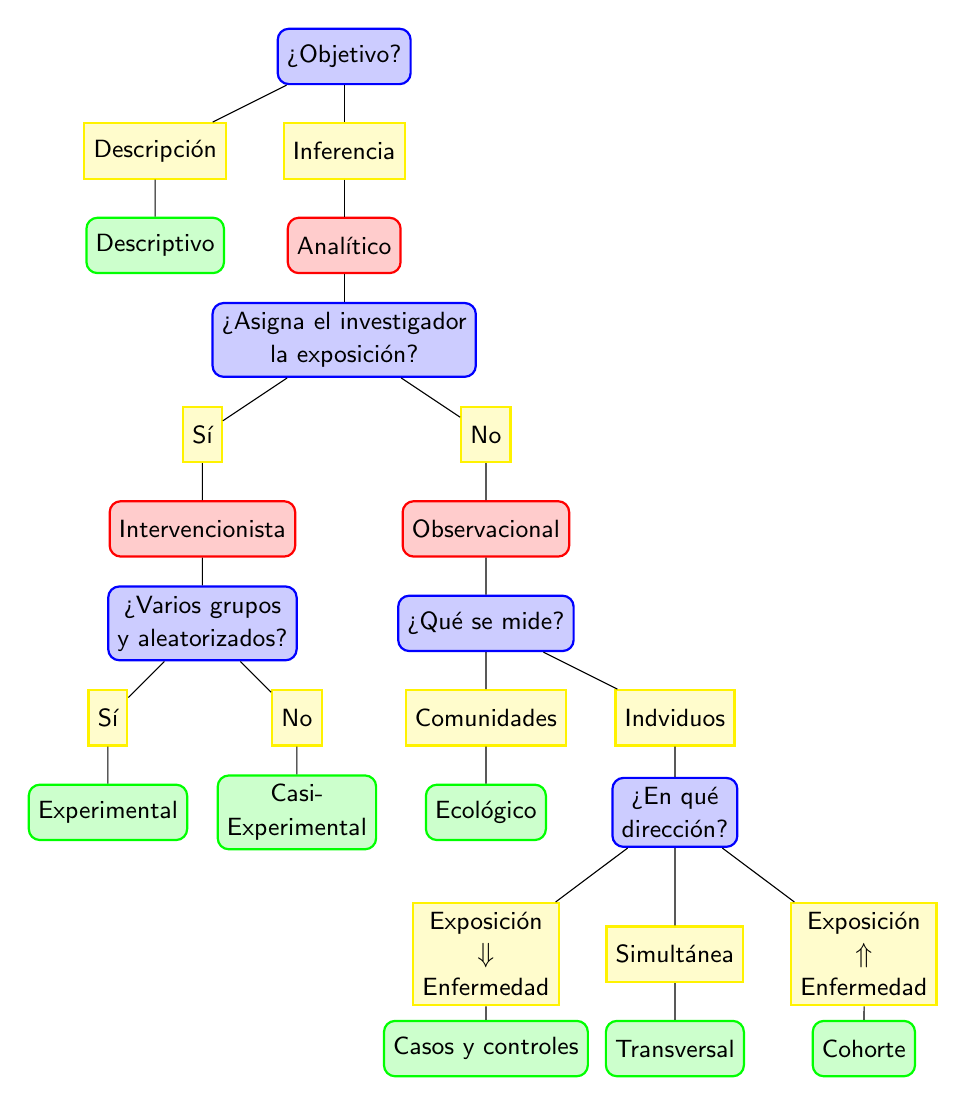
\begin{tikzpicture}[>=stealth,scale=1.2,
preg/.style ={rectangle, draw=blue, thick, fill=blue!20, align=center, rounded corners, minimum height=2em,},
resp/.style={rectangle, draw=yellow, thick, fill=yellow!20, align=center,  minimum height=2em},
study/.style={rectangle, draw=green, thick, fill=green!20, align=center, rounded corners,  minimum height=2em},
prestudy/.style={rectangle, draw=red, thick, fill=red!20, align=center,  minimum height=2em,rounded corners}]

\draw (0,3) node[preg] (P0) {\small\sf ¿Objetivo?};  
\draw (-2,2) node[resp] (Si0) {\small\sf Descripción};  
\draw (0,2) node[resp] (No0) {\small\sf Inferencia};  
\draw (-2,1) node[study] (Desc) {\small\sf Descriptivo};  
\draw (0,1) node[prestudy] (Anal) {\small\sf Analítico};  
\draw (0,0) node[preg] (P2) {\small\sf ¿Asigna el investigador\\ \small\sf la exposición?};  
\draw (-1.5,-1) node[resp] (Si2) {\small\sf Sí};  
\draw (1.5,-1) node[resp] (No2) {\small\sf No};  
\draw (-1.5,-2) node[prestudy] (Int) {\small\sf Intervencionista};  
\draw (1.5,-2) node[prestudy] (Obs) {\small\sf Observacional};  
\draw (-1.5,-3) node[preg] (P3) {\small\sf ¿Varios grupos\\ \small\sf y aleatorizados?};  
\draw (-2.5,-4) node[resp] (Si3) {\small\sf Sí};  
\draw (-0.5,-4) node[resp] (No3) {\small\sf No};  
\draw (-2.5,-5) node[study] (Exp) {\small\sf Experimental};  
\draw (-0.5,-5) node[study] (CExp) {\small\sf Casi-\\ \small \sf Experimental};  
\draw (1.5,-3) node[preg] (P1) {\small\sf ¿Qué se mide?};  
\draw (3.5,-4) node[resp] (RI) {\small\sf Indviduos};  
\draw (1.5,-4) node[resp] (RC) {\small\sf Comunidades};  
\draw (1.5,-5) node[study] (ES) {\small\sf Ecológico};  
\draw (3.5,-5) node[preg] (P5) {\small\sf ¿En qué\\ \small\sf dirección?};  
\draw (1.5,-6.5) node[resp] (RCC) {\small\sf Exposición\\ $\Downarrow$\\\small\sf  Enfermedad};  
\draw (3.5,-6.5) node[resp] (RTr) {\small\sf Simultánea};  
\draw (5.5,-6.5) node[resp] (RCo) {\small\sf Exposición\\ $\Uparrow$\\\small\sf  Enfermedad};  
\draw (1.5,-7.5) node[study] (CC) {\small\sf Casos y controles};  
\draw (3.5,-7.5) node[study] (Tr) {\small\sf Transversal};  
\draw (5.5,-7.5) node[study] (Co) {\small\sf Cohorte};  


\draw (P0)--(Si0);
\draw (P0)--(No0);


\draw (P2)--(Si2);
\draw (P2)--(No2);
\draw (Si2)--(Int);
\draw (No2)--(Obs);
\draw (Int)--(P3);
\draw (P3)--(Si3);
\draw (P3)--(No3);
\draw (Si3)--(Exp);
\draw (No3)--(CExp);
\draw (Obs)--(P1);
\draw (P1)--(RI);
\draw (P1)--(RC);
\draw (RC)--(ES);
\draw (RI)--(P5);
\draw (Si0)--(Desc);
\draw (No0)--(Anal);
\draw (Anal)--(P2);
\draw (P5)--(RCC);
\draw (P5)--(RTr);
\draw (P5)--(RCo);
\draw (RCC)--(CC);
\draw (RTr)--(Tr);
\draw (RCo)--(Co);


\end{tikzpicture}
\end{center}

\end{document}